% -*- mode: LaTeX -*-


% -*- mode: LaTeX; tex-command: "pdflatex" -*-

% $Id$




\documentclass[10pt,draft,a4paper]{book}
%\includeonly{s-cactus}
%\documentclass[draft,a4paper]{report}

%\usepackage{concrete}          % ok - legible
%\usepackage{beton}             % ok - legible
%\usepackage{times}             % ok - standard
%\usepackage{utopia}            % ok
\usepackage{charter}           % ok - very legible, good in PDF
%\usepackage{bookman}            % ok - legible while typing
%\usepackage{helvetic}          % no change
%\usepackage{palatino}          % ok - nice, like it
%\usepackage{lucidabr}          % No good, due to missing fonts here.
%\usepackage{a4wide}
\usepackage{fullpage}
\usepackage{isolatin1}
%\usepackage{parskip}
% \usepackage{draft}
\usepackage{alltt}
\usepackage{parskip}
\usepackage{varioref}           % gives better references
\usepackage{verbatim}
\usepackage{fancyhdr}           % provide headers where I can put the
                                % filenames.
\usepackage{color}
%\usepackage{myshowlocation}
\usepackage{graphicx}
%\usepackage[pdftex]{graphicx}
% hyperref breaks \vref :-(
% 
% \usepackage[%pdftex,
%   pdftitle={Database backed Websites},
%   pdfauthor={Thorbjoern Ravn Andersen},
%   pdfsubject={pdfsubject},
%   pdfkeywords={pdfkeywords},
%   pdfpagemode={UseOutlines},
%   pagebackref,hyperindex,,
%   bookmarks,bookmarksopen={false},
%   pdfstartview={FitH},
%   colorlinks,linkcolor={blue},citecolor={blue},
%   urlcolor={red}
% ]{hyperref}


%%%%%%%%%%%%%%%%%%%%%%%%%%%%%%%%%%%%%%%%%%%%%%%%%%%%%%%%%%%%
%
% new commands
%
% \framepage{15cm}{text}
\newcommand{\framepage}[2]{\begin{center}\fbox{\begin{minipage}{#1}#2
      \end{minipage}}\end{center}}

% \unixcommand{emacs}
\newcommand{\unixcommand}[1]{``\texttt{{#1}}''}
% \ntcommand{jview}
\newcommand{\ntcommand}[1]{``\texttt{{#1}}''}

% \texcommand{booh} -> \booh
\newcommand{\texcommand}[1]{\protect{\(\backslash\)}#1}

% \myurl{http://sunsite.auc.dk}{The Danish SunSite}
%\newcommand{\myurl}[2]{\begin{underline}{#2}\end{underline}\footnote{{#1}}}
%\newcommand{\myurl}[2]{\href{#1}{#2}}
% \hfil magic by Soeren Sandmann <sandmann@daimi.au.dk>
\newcommand{\myurl}[2]{{#2}\footnote{\ldots{#2}\ldots \hfil\penalty1000\hfilneg\hskip-5em\hbox{}\hskip5em%
{\tt #1}}}

% \tag{hr}  ->  <hr>
\newcommand{\tag}[1]{$<$#1$>$}

% \mycitation{what}{who}{where}
\newcommand{\mycitation}[3]{
  \begin{quotation}
    \textit{``{#1}''}

  {#2} -- {#3}
\end{quotation}}

% \myimage{filename}{Title}{reference}
% the if seperates between pdf and non pdf.
\newcommand{\myimage}[3]{
  \begin{figure}[htbp]
    \begin{center}
      
%       \ifx\pdfoutput\undefined
% % dvi
% %        [Graphic: \href{#1.png}{#1}]
%         \includegraphics[scale=0.4]{#1}
%       \else
% % pdf
%         \includegraphics[scale=0.4]{#1}
%       \fi
      \includegraphics[scale=0.5]{#1} 
      \caption{#2}
      \label{fig:#3}
    \end{center}
  \end{figure}
}

\newenvironment{my-detour}{\begin{quotation}\small}{\end{quotation}}


% \myinclude{foobar} - includes file and set top header
%\newcommand{\myinclude}[1]{\texttt{\lhead{#1}}\include{#1}\lhead{back from #1}}
% Trick from page 16 in fancyhdr documentation
\newcommand{\currentinputfile}{}
\newcommand{\myinclude}[1]{%
  \renewcommand{\currentinputfile}{File:\texttt{#1}}\include{#1}%
  \renewcommand{\currentinputfile}{}}


%%% Local Variables: 
%%% mode: latex
%%% TeX-master: "rapport"
%%% End: 


%%%%%%%%%%%%%%%%%%%%%%%%%%%%%%%%%%%%%%%%%%%%%%%%%%%%%%%%%%%%

% Here we go!

%%%%%%%%%%%%%%%%%%%%%%%%%%%%%%%%%%%%%%%%%%%%%%%%%%%%%%%%%%%%

\author{Thorbj{\o}rn Ravn Andersen}

\title{{\Huge \textbf{Database backed Websites}} \\
  Dynamic Webpublishing with XML\\ 
  \textit{D R A F T -- $ $Revision$ $}} % Math hack for RCS

%\bibliographystyle{alpha}
\bibliographystyle{plainnat}

% While writing - this provides fileinformation on includes
\lhead{\currentinputfile}
\pagestyle{fancy}
%
% allow C-c C-f C-f to be easy shortcut to standout text
%\renewcommand{\textsl}[1]{\colorbox{black}{{\textcolor{white}#1}}}
\renewcommand{\textsf}[1]{\fbox{{\sl{#1}}}}

% End.

\begin{document}

\myinclude{s-front-matter}
\myinclude{s-introduction}
\myinclude{s-terms-and-concepts}
\myinclude{s-dynamically-generated-documents}
\myinclude{s-standards}
\myinclude{s-sample-websites}
\myinclude{s-xml}
\myinclude{s-docbook}
\myinclude{s-sql}
\myinclude{s-users-transparently}
\myinclude{s-active-and-passive-data-acquisition}
\myinclude{s-search-engines-and-data-mining}
\myinclude{s-available-technologies}
\myinclude{s-cactus}
\myinclude{s-conclusion}
\appendix
\myinclude{s-konsensus}


\myinclude{s-tex-and-latex}
\myinclude{s-report-writing-tools}

%\section{Available hardware and software}
\myinclude{s-available-hardware-and-software}
\section{Bibliography with Web references}
Full reference with a lot of annotated URL's.



%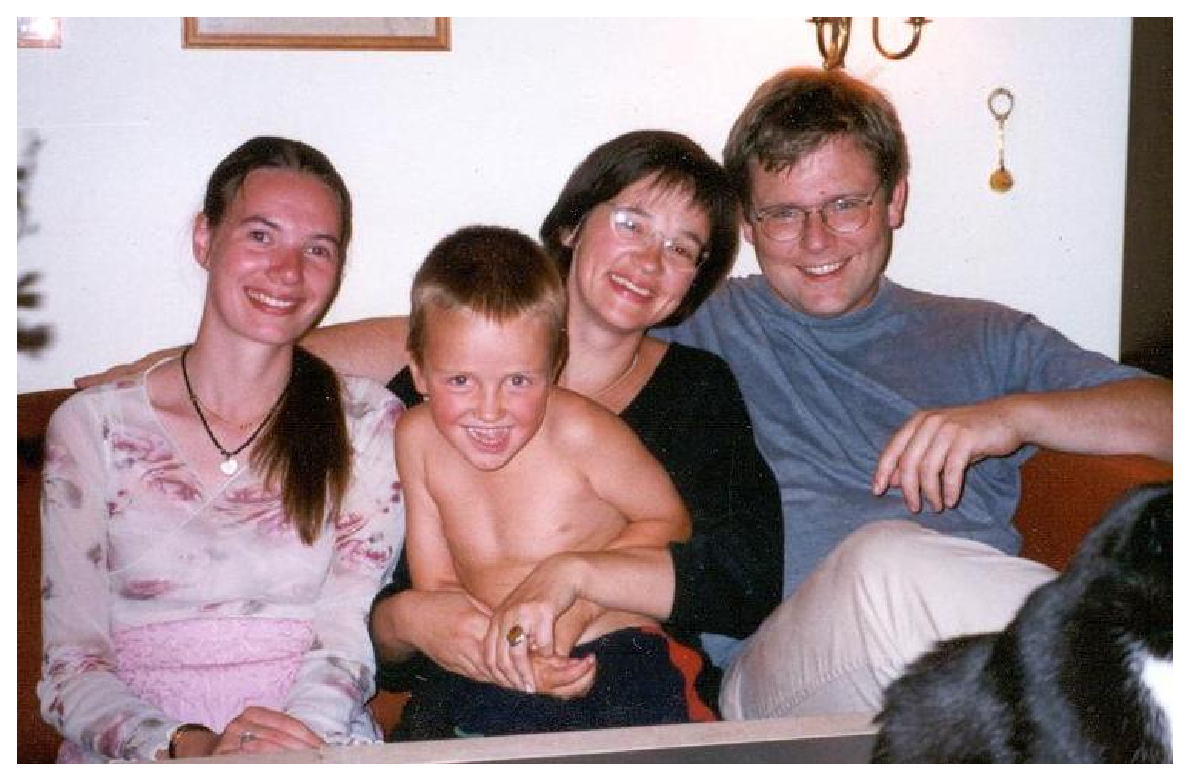
\includegraphics{gr/familie}
\bibliography{books}

\tableofcontents

\section{Cross references to this page have not been inserted at the
  correct page}

\label{fig:slashdot-1}
\label{sec:CGI-modperl}
\label{sec:CGI-php3}
\label{sec:CGI-servlets}
\label{fig:mip-recently-changed-pages}
\label{sec:html-meta-tags}
\label{cha:on-demand-rendering}
\label{sec:emacs-with-psgml}
\label{sec:java-servlets}

\section{The importance of a web cache}
\label{sec:the-importance-of-a-web-cache}

A database query is expensive, and it requires an expert to tune the
database to run as fast as possible.  It is not, however, always
necessary to have the webserver do a database query to serve a page -
often the generated page is valid for a short or long term period,
and then it is relatively easy to cache the page for this period.

Here is one way to do it:

\begin{itemize}
\item Configure the script generating the page, to add an
  ``\texttt{Expires''} header with a reasonable time of expiry
\item Set up squid (\vref{sec:squid}) in http-accellerator mode, where
  it transparently adds cache facilities to a webserver, respecting
  the ``\texttt{Expires}'' header.
\end{itemize}


Mangler:

\begin{itemize}
\item myurl footsnotes - urls should be broken if too long, numbers
  should perhaps not be reset at new chapters, slightly smaller bottom
  margin 
  
  
  
\item myimage maa gerne hyperlinke til tiff eller pngfil i
  hyperudgaven?  ER det muligt?
\item tal med sm om internetbibliotekarer
\item afsnit om filosofi/osv med brugernes egne vaerktoejer til at
  lave sgml dokumenter.

  
\end{itemize}
\mycitation{The devil is real.  He lives inside C programs.}{Phillip
  Greenspun}{\cite{phillipandalexsguidetowebpublishing} page 202}


\end{document}

%
% and all that was ever heard from him again, was the sound of Tubular Bells! 
%
% %%%%%%%%%%%%%%%%%%%%%%%%%%%%%%%%%%%%%%%%%%%%%%%%%%%%%%%%%%%%%%%%%%%%%%%%%%%

